\documentclass[compress]{beamer}
\mode<presentation>
{
 \usetheme{Vilanova}
}

\usepackage[english]{babel}

\usepackage[utf8]{inputenc}

\usepackage{times}
\usepackage[T1]{fontenc}

\usepackage{amsfonts}
\usepackage{amsmath}
\usepackage{amssymb}
\usepackage{tikz}
\usepackage{eurosym}
%\usepackage{url}
\usepackage[normal]{subfigure}
\newcommand{\goodgap}{%
	\hspace{\subfigtopskip}%
	\hspace{\subfigbottomskip}}



%\newtheorem{definition}{Definition}

\title{Traitement d'images de télédétection}

\subtitle{La main à la pâte avec OTB/Monteverdi} % (optional)


\author
{jordi.inglada@cesbio.cnes.fr}
\normalsize

\institute[Cesbio] % (optional, but mostly needed)
{\textsc{Centre d'Études Spatiales de la Biosphère, Toulouse, France}}

\date{}

\pgfdeclareimage[height=96mm,width=128mm]{background}{fondsClairSansLogo}
\setbeamertemplate{background}{\pgfuseimage{background}}
\pgfdeclareimage[height=0.6cm]{logoIncrust}{logoIncrust}
\pgfdeclareimage[height=0.5cm]{logo_cesbio}{logo_cesbio}
\logo{
\begin{tabular}{lp{0.25\textwidth}lp{0.25\textwidth}r}
\href{http://www.cesbio.ups-tlse.fr/}{\pgfuseimage{logo_cesbio}}
&&\footnotesize{AUF - Marrakech 2011}&&
\href{http://www.orfeo-toolbox.org}{\pgfuseimage{logoIncrust}}\\
\end{tabular}
}


\subject{Orfeo Toolbox}

% Delete this, if you do not want the table of contents to pop up at
% the beginning of each subsection:
\AtBeginSection[]
{
  \begin{frame}<beamer>
    \frametitle{Plan}
%     \tableofcontents[currentsection,currentsubsection]
\vspace*{-0.5cm}
    \tableofcontents[currentsection]
  \end{frame}
}




% If you wish to uncover everything in a step-wise fashion, uncomment
% the following command: 

% \beamerdefaultoverlayspecification{<+->}

\begin{document}

\begin{frame}
  \titlepage
  \begin{center}
{\tiny Ce contenu est dérivé de la formation \href{http://www.orfeo-toolbox.org/packages/PragmaticRemoteSensing-handout.pdf}{``Pragmatic Remote
  Sensing''} dispensée par J. Inglada et E. Christophe en juillet 2010
  dans le cadre du colloque IGARSS. Il est mis à disposition selon les termes de la licence :\\
Creative Commons Paternité – Partage à l’Identique 3.0 non transcrit.} \href{http://creativecommons.org/licenses/by-sa/3.0/}{
\includegraphics[width=0.05\textwidth]{/home/inglada/Dev/GH/IGARSS2010/Tutorial/Slides/Ressources/CC-licence.png}}    
  \end{center}

\end{frame}

\begin{frame}
\frametitle{Why?}
\begin{block}{Common problems}
\begin{itemize}
 \item Reading images
 \item Accessing metadata
 \item Implementing state of the art algorithms
\end{itemize}
\end{block}
$\Rightarrow$ to be able to \alert{extract the most information}, we
 need to \alert{use the best} of what is available: data, algorithms,\ldots
\end{frame}


\section{Introduction to the Orfeo Toolbox}



\subsection[What]{What is it?}
\begin{frame}
\frametitle{What is Orfeo Toolbox (OTB)?}

\textbf{In the frame of CNES ORFEO Program}
\begin{alertblock}{Goal}
Make the development of new algorithms and their validation easier
\end{alertblock}
\begin{block}{}
\begin{itemize}
 \item C++ library: provide many algorithms (pre-processing, image analysis) with a common interface
 \item Open-source: free to use, to modify, you can make your own software based on OTB and sell it
 \item Multiplatform: Windows, Linux, Unix, Mac
\end{itemize}
\end{block}
\end{frame}


\subsection[When]{A bit of history}
% start
% applications apparition
% current value
\begin{frame}
\frametitle{A bit of History}
\begin{block}{Everything begins (2006)}
\scriptsize
\begin{itemize}
 \item Started in 2006 by CNES (French Space Agency), funding \alert{several full-time developers}
 \item Targeted at high resolution images (Pleiades to be launched in 2010) but with application to other sensors
 \item 4 year budget, over 1,000,000\euro~recently renewed for 1 additional
       year (500,000\euro)
\end{itemize}
\end{block}
\begin{block}{Moving to user friendly applications (2008)}
\scriptsize
\begin{itemize}
  \item Strong interactions with the end-user community highlighted that \alert{applications for non-programmers} are important
  \item Several applications for non programmers (with GUI) since early 2008
  \item Several training courses (3/5-day courses) given in France, Belgium,
        Madagascar, UNESCO and now Hawaii
\end{itemize}
\end{block}
\end{frame}


\subsection[Why]{Why doing that?}
%make sure satellite images are used
\begin{frame}
\frametitle{Why doing that?}
\begin{overprint}
\onslide<1->{
\begin{block}{Is it successful so far?}
\scriptsize
\begin{itemize}
  \item OTB user community \alert{growing steadily} (programmers and application users)
  \item Presented at IGARSS and ISPRS in 2008, special session in IGARSS in 2009
  \item CNES is planning to extend the budget for several more years
  \item Value analysis is very positive (cf. \href{http://www.ohloh.net/p/otb}{Ohloh}): \alert{re-using is powerful}
\end{itemize}
\end{block}
}
\onslide<2->{
\begin{block}{Why make a multi-million dollar software and give it for free?}
\scriptsize
\begin{itemize}
 \item CNES is not a software company
 \item One goal is to \alert{encourage research}: it is critical for researchers to know what is in the box
 \item CNES makes satellites and wants to make sure the \alert{images are used}
 \item if more people have the tools to use satellite images, it is good for CNES
\end{itemize}
\end{block}
}
\end{overprint}
\end{frame}


\subsection[How]{How?}
% Using other library
\begin{frame}
\frametitle{How?}
\begin{overprint}
\onslide<1->{
\begin{block}{How to reach this goal?}
Using the best work of others: do not reinvent the wheel
\end{block}
}
\onslide<2->{
\begin{block}{Many open-source libraries of good quality}
\scriptsize
\begin{itemize}
  \item ITK: software architecture (streaming, multithreading), many image processing algorithms
 \item Gdal/Ogr: reading data format (geotiff, raw, png, jpeg, shapefile, \ldots)
 \item Ossim: sensor models (Spot, RPC, SAR, \ldots) and map projections
 \item 6S: radiometric corrections
 \item and many other: libLAS (lidar data), Edison (Mean Shift clustering), libSiftFast (SIFT), Boost (graph), libSVM (Support Vector Machines)
\end{itemize}
\normalsize
\alert{$\Rightarrow$ all behind a common interface}
\end{block}
}
\end{overprint}
\end{frame}


\section{Applications and librairy}
\begin{frame}
\frametitle{Application}
\begin{block}{Currently}
\scriptsize
\begin{itemize}
 \item Image viewer
 \item Image Segmentation
 \item Image Classification (by SVM)
 \item Land Cover
 \item Feature Extraction
 \item Road Extraction
 \item Orthorectification (with Pan Sharpening)
 \item Fine registration
 \item Image to database registration
 \item Object counting
 \item Urban area detection
 \item more to come
\end{itemize}
\end{block}
\end{frame}



% - functionalities
% - some technical details
% - doc
% - binding

\subsection{Components}

\begin{frame}
\frametitle{Components available}
 \begin{block}{Currently}
\scriptsize
\begin{itemize}
\item Most satellite image formats
\item Geometric corrections
\item Radiometric corrections
\item Change detection
\item Feature extraction
\item Classification
\end{itemize}
\end{block}


 \begin{block}{Huge documentation available}
\scriptsize
\begin{itemize}
\item Software Guide (+600 pages pdf), also the \href{http://www.orfeo-toolbox.org/SoftwareGuide/}{online version}
\item \href{http://www.orfeo-toolbox.org/doxygen}{Doxygen}: documentation for developers
\end{itemize}
\end{block}
\end{frame}

\subsection{Architecture}

\begin{frame}
 \frametitle{A powerful architecture}
  \begin{block}{Modular}
\scriptsize
\begin{itemize}
\item Easy to combine different blocks to do new processing
\end{itemize}
\end{block}
  \begin{block}{Scalable}
\scriptsize
\begin{itemize}
\item Streaming (processing huge images on the flow) transparent for the user of the library
\item Multithreading (using multicore CPUs) also
\end{itemize}
\end{block}
\end{frame}

\subsection[But]{But steep learning}

\begin{frame}
\setbeamercovered{invisible} 
\frametitle{But a steep learning curve for the programmer}
\begin{overprint}
\onslide<1->{
\begin{block}{Advanced programming concepts}
\scriptsize
\begin{itemize}
\item Template metaprogramming (generic programming)
\item Design patterns (Factory, Functors, Smart Pointers, ...)
\end{itemize}
\end{block}
}
\onslide<2->{
\centering Steep learning curve
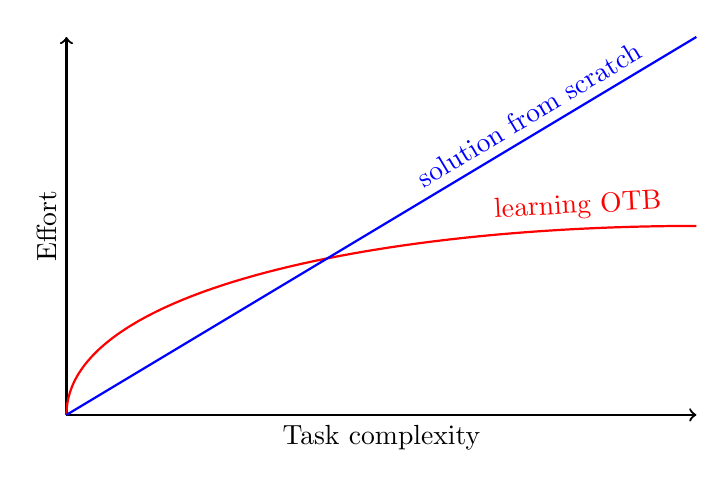
\begin{tikzpicture}[thick,scale=0.8]

\node (origin) at (0,0){};
\draw[->] (0,0) -- node[sloped,below]{Task complexity}(10,0);
\draw[->] (0,0) -- node[sloped,above]{Effort}(0,6);

\draw[red] (0,0) .. controls +(up:20mm) and +(left:50mm)
            .. node[very near end,sloped,above]{learning OTB} (10,3);
\draw[blue] (0,0) -- node[near end,sloped,above]{solution from scratch}(10,6);
\end{tikzpicture}

}
  \end{overprint}
\end{frame}


\begin{frame}
\frametitle{Ask questions}
\begin{block}{As for everything: easier when you're not alone}
\scriptsize
\begin{itemize}
\item Much easier if you have somebody around to help!
\item We didn't know anything not so long ago...
\item Not surprising that most software companies now focus their offer on support: help is important
\end{itemize}
\end{block}
\end{frame}
     


\subsection{Monteverdi}
\begin{frame}
\frametitle{Making it easier for the users: Monteverdi}
\begin{columns}
\begin{column}{0.5\textwidth}
\begin{block}{Module architecture}
\scriptsize
\begin{itemize}
\item Standard input/output
\item Easy to customize for a specific purpose
\item Full streaming or caching the data
\item Each module follows a MVC pattern
\end{itemize}
\end{block}
\end{column}
\begin{column}{0.5\textwidth}
\begin{figure}[]
  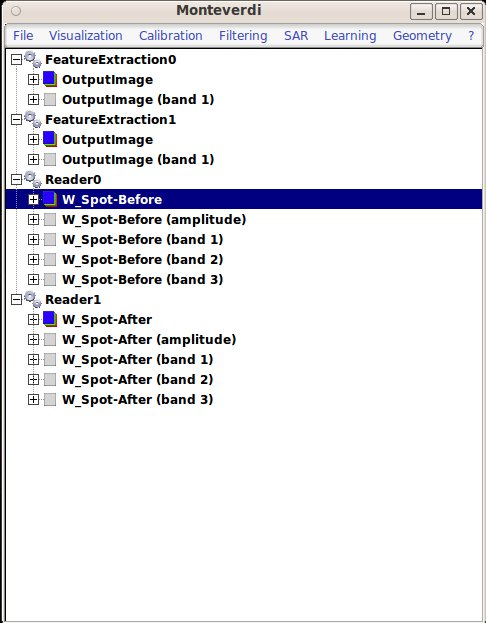
\includegraphics[width=0.9\textwidth]{monteverdi1.jpg}
\end{figure}
\end{column}
\end{columns}
\end{frame}

\begin{frame}
\frametitle{Making it easier for the users: Monteverdi}
\begin{figure}[]
  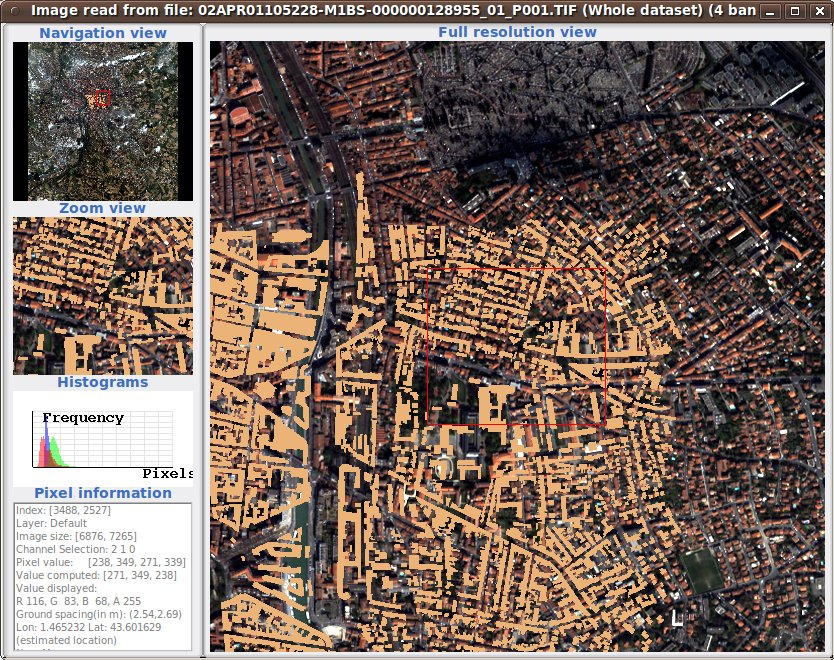
\includegraphics[width=0.8\textwidth]{monteverdi2.jpg}
\end{figure}
\end{frame}

\subsection{Bindings}
\begin{frame}
\frametitle{Bindings: access through other languages}
\begin{block}{Not everybody uses C++!}
\scriptsize
\begin{itemize}
\item Bindings provide an access to the library through other languages
\item \alert{Python}: available
\item \alert{Java}: available
\item \alert{IDL/Envi}: cooperation with ITT VIS to provide a method
  to access OTB through idl/envi (working but no automatic generation)
  \item \alert{Matlab}: recent user contribution (R. Bellens from TU Delft)
\item Other languages supported by Cable Swig might be possible (Tcl, Ruby?)
\end{itemize}
\end{block}
\end{frame}

\end{document}
